% Options for packages loaded elsewhere
\PassOptionsToPackage{unicode}{hyperref}
\PassOptionsToPackage{hyphens}{url}
%
\documentclass[
]{article}
\usepackage{lmodern}
\usepackage{amssymb,amsmath}
\usepackage{ifxetex,ifluatex}
\ifnum 0\ifxetex 1\fi\ifluatex 1\fi=0 % if pdftex
  \usepackage[T1]{fontenc}
  \usepackage[utf8]{inputenc}
  \usepackage{textcomp} % provide euro and other symbols
\else % if luatex or xetex
  \usepackage{unicode-math}
  \defaultfontfeatures{Scale=MatchLowercase}
  \defaultfontfeatures[\rmfamily]{Ligatures=TeX,Scale=1}
\fi
% Use upquote if available, for straight quotes in verbatim environments
\IfFileExists{upquote.sty}{\usepackage{upquote}}{}
\IfFileExists{microtype.sty}{% use microtype if available
  \usepackage[]{microtype}
  \UseMicrotypeSet[protrusion]{basicmath} % disable protrusion for tt fonts
}{}
\makeatletter
\@ifundefined{KOMAClassName}{% if non-KOMA class
  \IfFileExists{parskip.sty}{%
    \usepackage{parskip}
  }{% else
    \setlength{\parindent}{0pt}
    \setlength{\parskip}{6pt plus 2pt minus 1pt}}
}{% if KOMA class
  \KOMAoptions{parskip=half}}
\makeatother
\usepackage{xcolor}
\IfFileExists{xurl.sty}{\usepackage{xurl}}{} % add URL line breaks if available
\IfFileExists{bookmark.sty}{\usepackage{bookmark}}{\usepackage{hyperref}}
\hypersetup{
  pdftitle={One-sample t-toets},
  hidelinks,
  pdfcreator={LaTeX via pandoc}}
\urlstyle{same} % disable monospaced font for URLs
\usepackage[margin=1in]{geometry}
\usepackage{color}
\usepackage{fancyvrb}
\newcommand{\VerbBar}{|}
\newcommand{\VERB}{\Verb[commandchars=\\\{\}]}
\DefineVerbatimEnvironment{Highlighting}{Verbatim}{commandchars=\\\{\}}
% Add ',fontsize=\small' for more characters per line
\usepackage{framed}
\definecolor{shadecolor}{RGB}{248,248,248}
\newenvironment{Shaded}{\begin{snugshade}}{\end{snugshade}}
\newcommand{\AlertTok}[1]{\textcolor[rgb]{0.94,0.16,0.16}{#1}}
\newcommand{\AnnotationTok}[1]{\textcolor[rgb]{0.56,0.35,0.01}{\textbf{\textit{#1}}}}
\newcommand{\AttributeTok}[1]{\textcolor[rgb]{0.77,0.63,0.00}{#1}}
\newcommand{\BaseNTok}[1]{\textcolor[rgb]{0.00,0.00,0.81}{#1}}
\newcommand{\BuiltInTok}[1]{#1}
\newcommand{\CharTok}[1]{\textcolor[rgb]{0.31,0.60,0.02}{#1}}
\newcommand{\CommentTok}[1]{\textcolor[rgb]{0.56,0.35,0.01}{\textit{#1}}}
\newcommand{\CommentVarTok}[1]{\textcolor[rgb]{0.56,0.35,0.01}{\textbf{\textit{#1}}}}
\newcommand{\ConstantTok}[1]{\textcolor[rgb]{0.00,0.00,0.00}{#1}}
\newcommand{\ControlFlowTok}[1]{\textcolor[rgb]{0.13,0.29,0.53}{\textbf{#1}}}
\newcommand{\DataTypeTok}[1]{\textcolor[rgb]{0.13,0.29,0.53}{#1}}
\newcommand{\DecValTok}[1]{\textcolor[rgb]{0.00,0.00,0.81}{#1}}
\newcommand{\DocumentationTok}[1]{\textcolor[rgb]{0.56,0.35,0.01}{\textbf{\textit{#1}}}}
\newcommand{\ErrorTok}[1]{\textcolor[rgb]{0.64,0.00,0.00}{\textbf{#1}}}
\newcommand{\ExtensionTok}[1]{#1}
\newcommand{\FloatTok}[1]{\textcolor[rgb]{0.00,0.00,0.81}{#1}}
\newcommand{\FunctionTok}[1]{\textcolor[rgb]{0.00,0.00,0.00}{#1}}
\newcommand{\ImportTok}[1]{#1}
\newcommand{\InformationTok}[1]{\textcolor[rgb]{0.56,0.35,0.01}{\textbf{\textit{#1}}}}
\newcommand{\KeywordTok}[1]{\textcolor[rgb]{0.13,0.29,0.53}{\textbf{#1}}}
\newcommand{\NormalTok}[1]{#1}
\newcommand{\OperatorTok}[1]{\textcolor[rgb]{0.81,0.36,0.00}{\textbf{#1}}}
\newcommand{\OtherTok}[1]{\textcolor[rgb]{0.56,0.35,0.01}{#1}}
\newcommand{\PreprocessorTok}[1]{\textcolor[rgb]{0.56,0.35,0.01}{\textit{#1}}}
\newcommand{\RegionMarkerTok}[1]{#1}
\newcommand{\SpecialCharTok}[1]{\textcolor[rgb]{0.00,0.00,0.00}{#1}}
\newcommand{\SpecialStringTok}[1]{\textcolor[rgb]{0.31,0.60,0.02}{#1}}
\newcommand{\StringTok}[1]{\textcolor[rgb]{0.31,0.60,0.02}{#1}}
\newcommand{\VariableTok}[1]{\textcolor[rgb]{0.00,0.00,0.00}{#1}}
\newcommand{\VerbatimStringTok}[1]{\textcolor[rgb]{0.31,0.60,0.02}{#1}}
\newcommand{\WarningTok}[1]{\textcolor[rgb]{0.56,0.35,0.01}{\textbf{\textit{#1}}}}
\usepackage{graphicx,grffile}
\makeatletter
\def\maxwidth{\ifdim\Gin@nat@width>\linewidth\linewidth\else\Gin@nat@width\fi}
\def\maxheight{\ifdim\Gin@nat@height>\textheight\textheight\else\Gin@nat@height\fi}
\makeatother
% Scale images if necessary, so that they will not overflow the page
% margins by default, and it is still possible to overwrite the defaults
% using explicit options in \includegraphics[width, height, ...]{}
\setkeys{Gin}{width=\maxwidth,height=\maxheight,keepaspectratio}
% Set default figure placement to htbp
\makeatletter
\def\fps@figure{htbp}
\makeatother
\setlength{\emergencystretch}{3em} % prevent overfull lines
\providecommand{\tightlist}{%
  \setlength{\itemsep}{0pt}\setlength{\parskip}{0pt}}
\setcounter{secnumdepth}{-\maxdimen} % remove section numbering

\title{One-sample t-toets}
\author{}
\date{\vspace{-2.5em}}

\begin{document}
\maketitle

{
\setcounter{tocdepth}{2}
\tableofcontents
}
\begin{verbatim}
<div class="navbar-header">
  <button type="button" class="navbar-toggle collapsed" data-toggle="collapse" data-target="#navbar">
    <span class="icon-bar"></span>
    <span class="icon-bar"></span>
    <span class="icon-bar"></span>
  </button>
  <a class="navbar-brand" href="Index.html">Statistisch Handboek Studiedata</a>
</div>
<div id="navbar" class="navbar-collapse collapse">
  <ul class="nav navbar-nav navbar-start">
    <li>
\end{verbatim}

Toetsmatrix (R)

Toetsmatrix (Python)

Begrippenlijst

Over

Verantwoording

Feedback

Nieuwsbrief

\begin{verbatim}
  </ul>
  <ul class="nav navbar-nav navbar-right">

  </ul>
</div><!--/.nav-collapse -->
\end{verbatim}

Disclaimer: Het peer review proces voor deze toets is nog niet afgerond;
daarom is deze pagina nog in concept.

\hypertarget{toepassing}{%
\section{Toepassing}\label{toepassing}}

Gebruik de \emph{one sample t-toets} om het gemiddelde van de steekproef
te vergelijken met een bekend gemiddelde of norm van de totale
populatie.\footnote{Van Geloven, N. (25 mei 2016). \emph{T-toets}
  \href{https://wikistatistiek.amc.nl/index.php/T-toets\#one_sample_t-toets}{Wiki
  Statistiek Academisch Medisch Centrum}.}

\hypertarget{onderwijscasus}{%
\section{Onderwijscasus}\label{onderwijscasus}}

\leavevmode\hypertarget{casus}{}%
De opleidingsdirecteur van de opleiding Werktuigbouwkunde wil weten of
het gemiddelde eindexamencijfer voor de exacte vakken (Wiskunde,
Natuurkunde en Scheikunde; WNS) van vwo studenten anders is dan het
landelijk gemiddelde (6,8).\footnote{Centraal Instituut voor
  Toetsontwikkeling (2018). \emph{Examenverslag 2018}.
  \url{https://www.cito.nl/onderwijs/voortgezet-onderwijs/centrale-examens-voortgezet-onderwijs/tools-en-informatie-voor-docenten/examenverslagen/examenverslag-2018}}
Met deze gegevens probeert zij een inschatting te maken van het niveau
van de studenten en kan zij bepalen of het curriculum van de inleidende
vakken genoeg aansluit bij eerstejaars studenten met een vwo
vooropleiding.

Dit onderzoek vertaalt zich in de volgende combinatie van hypothesen,
waarbij de nulhypothese zo geformuleerd is dat er geen effect is en de
alternatieve hypothese zo geformuleerd is dat er een effect is wat
overeenkomt met de verwachting van de onderzoeker.

\emph{H\textsubscript{0}}: Het gemiddelde eindexamencijfer voor de
exacte vakken van vwo studenten die beginnen aan de Bachelor
Werktuigbouwkunde is gelijk aan het landelijk gemiddelde: µ = 6,8.

\emph{H\textsubscript{A}}: Het gemiddelde eindexamencijfer voor de
exacte vakken van vwo studenten die beginnen aan de Bachelor
Werktuigbouwkunde is anders dan het landelijk gemiddelde: µ ≠ 6,8.

\hypertarget{assumpties}{%
\section{Assumpties}\label{assumpties}}

Om een valide resultaat te bereiken moeten, voordat de toets kan worden
uitgevoerd, de data aan een aantal voorwaarden voldoen.

\hypertarget{normaliteit}{%
\subsection{Normaliteit}\label{normaliteit}}

De \emph{t-toets} gaat ervan uit dat de data van de steekproef normaal
verdeeld zijn. Ga er bij meer dan 100 observaties vanuit dat de t-toets
robuust genoeg is om uit te voeren zonder dat de data een normale
verdeling volgen.\footnote{Lumley, T., Diehr, P., Emerson, S., \& Chen,
  L. (2002). The importance of the normality assumption in large public
  health data sets. Annu Rev Public Health, 23, 151-69. doi:
  10.1146/annurev.publheath.23.100901.140546
  \url{http://rctdesign.org/techreports/arphnonnormality.pdf}}

Controleer de assumptie van normaliteit met de volgende stappen:\\
1. Controleer de data visueel met een histogram, een boxplot of een Q-Q
plot.\\
2. Toets of de data normaal verdeeld zijn met de
\emph{Kolmogorov-Smirnov test} of bij een kleinere steekproef (n
\textless{} 50) met de \emph{Shapiro-Wilk test}.\footnote{Laerd
  statistics (2018).
  \href{https://statistics.laerd.com/spss-tutorials/testing-for-normality-using-spss-statistics.php}{Testing
  for Normality using SPSS Statistics}.}, \footnote{Normaliteit. (14
  juli 2014).
  \href{https://wiki.uva.nl/methodologiewinkel/index.php/Normaliteit}{UvA
  Wiki Methodologiewinkel}.}

Als blijkt dat de data niet normaal verdeeld zijn, transformeer dan de
data eventueel en bepaal daarna of deze wel normaal verdeeld
zijn.\footnote{Bereken de logaritme van de variabele en de inverse (1
  gedeeld door de variabele), en bekijk of deze normaal verdeeld zijn.
  Als dat zo is, mag je die gebruiken voor de analyse.}

Als er geen sprake is van normaliteit, gebruik de
\href{07-Wilcoxon-signed-rank-toets-R.html}{Wilcoxon signed rank
toets}.\footnote{De \href{07-Wilcoxon-signed-rank-toets-R.html}{Wilcoxon
  signed rank toets} maakt een rangschikking van de data. Hierdoor is de
  test verdelingsvrij en is normaliteit geen assumptie. Ook zijn
  uitbijters minder van invloed op het eindresultaat. Toch wordt er voor
  deze test minder vaak gekozen, doordat bij het maken van een
  rankschikking de data informatie verliest. Als de data wel normaal
  verdeeld zijn heeft de
  \href{07-Wilcoxon-signed-rank-toets-R.html}{Wilcoxon signed rank
  toets} minder onderscheidend vermogen dan wanneer de \emph{one sample
  t-toets} uitgevoerd zou worden.}, \footnote{Prabhakaran, S.
  (2016-2017). \emph{Statistical Tests}.
  \url{http://r-statistics.co/Statistical-Tests-in-R.html}}

\hypertarget{uitvoering}{%
\section{Uitvoering}\label{uitvoering}}

Er is een dataset ingeladen met de gemiddelde eindexamencijfers van WNS
van eerstejaars Werktuigbouwkunde: \texttt{Gemiddeld\_cijfer\_WNS}.

\hypertarget{de-data-bekijken}{%
\subsection{De data bekijken}\label{de-data-bekijken}}

Gebruik \texttt{head()} en \texttt{tail()} om de structuur van de data
te bekijken.

\begin{Shaded}
\begin{Highlighting}[]
\CommentTok{## Eerste 5 observaties}
\KeywordTok{head}\NormalTok{(Gemiddeld_cijfer_WNS)}
\CommentTok{## [1] 7.400000 7.366667 7.366667 7.666667 5.933333 6.500000}

\CommentTok{## Laatste 5 observaties}
\KeywordTok{tail}\NormalTok{(Gemiddeld_cijfer_WNS)}
\CommentTok{## [1] 6.333333 6.133333 8.066667 5.166667 7.700000 6.366667}
\end{Highlighting}
\end{Shaded}

Inspecteer de data met \texttt{length()}, \texttt{mean()}en
\texttt{sd()} om meer inzicht te krijgen in de data.

\begin{Shaded}
\begin{Highlighting}[]
\CommentTok{## Gemiddelde en standaarddeviatie}
\KeywordTok{length}\NormalTok{(Gemiddeld_cijfer_WNS)}
\CommentTok{## [1] 124}
\KeywordTok{mean}\NormalTok{(Gemiddeld_cijfer_WNS)}
\CommentTok{## [1] 7.128763}
\KeywordTok{sd}\NormalTok{(Gemiddeld_cijfer_WNS)}
\CommentTok{## [1] 0.7850378}
\end{Highlighting}
\end{Shaded}

\begin{itemize}
\tightlist
\item
  Gemiddeld cijfer WNS (standaardafwijking): 7,13 (0,79). \emph{n} =
  124. 
\end{itemize}

\hypertarget{visuele-inspectie-van-normaliteit}{%
\subsection{Visuele inspectie van
normaliteit}\label{visuele-inspectie-van-normaliteit}}

Geef de verdeling van de data visueel weer met een histogram, Q-Q plot
en boxplot.

\hypertarget{histogram}{%
\subsubsection{Histogram}\label{histogram}}

Focus bij het analyseren van een histogram op de symmetrie van de
verdeling, de hoeveelheid toppen (modaliteit) en mogelijke uitbijters.
Een normale verdeling is symmetrisch, heeft één top en geen
uitbijters.\footnote{Outliers (13 augustus 2016).
  \href{https://wiki.uva.nl/methodologiewinkel/index.php/Outliers}{UvA
  Wiki Methodologiewinkel}.}, \footnote{Uitbijters kunnen bepalend zijn
  voor de uitkomst van toetsen. Bekijk of de uitbijters valide
  uitbijters zijn en niet een meetfout of op een andere manier incorrect
  verkregen data. Het weghalen van uitbijters kan de uitkomst ook
  vertekenen, daarom is het belangrijk om verwijderde uitbijters te
  melden in een rapport.}

\begin{Shaded}
\begin{Highlighting}[]
\CommentTok{## Histogram met ggplot2}
\KeywordTok{library}\NormalTok{(ggplot2)}

\KeywordTok{ggplot}\NormalTok{(}\KeywordTok{data.frame}\NormalTok{(Gemiddeld_cijfer_WNS), }
       \KeywordTok{aes}\NormalTok{(}\DataTypeTok{x =}\NormalTok{ Gemiddeld_cijfer_WNS)) }\OperatorTok{+}
\StringTok{  }\KeywordTok{geom_histogram}\NormalTok{(}\KeywordTok{aes}\NormalTok{(}\DataTypeTok{y =}\NormalTok{ ..density..),}
                 \DataTypeTok{binwidth =} \FloatTok{0.5}\NormalTok{, }
                 \DataTypeTok{color =} \StringTok{"white"}\NormalTok{, }
                 \DataTypeTok{fill =} \StringTok{"#158CBA"}\NormalTok{) }\OperatorTok{+}
\StringTok{  }\KeywordTok{geom_density}\NormalTok{(}\DataTypeTok{alpha =} \FloatTok{.2}\NormalTok{, }\DataTypeTok{adjust =} \DecValTok{1}\NormalTok{) }\OperatorTok{+}
\StringTok{  }\KeywordTok{ylab}\NormalTok{(}\StringTok{"Frequentiedichtheid"}\NormalTok{) }\OperatorTok{+}
\StringTok{  }\KeywordTok{xlab}\NormalTok{(}\StringTok{"Gemiddeld_cijfer_WNS"}\NormalTok{) }\OperatorTok{+}
\StringTok{  }\KeywordTok{scale_x_continuous}\NormalTok{(}\DataTypeTok{labels =} \KeywordTok{as.character}\NormalTok{(}\KeywordTok{seq}\NormalTok{(}\FloatTok{5.5}\NormalTok{, }\DecValTok{9}\NormalTok{, }\FloatTok{0.5}\NormalTok{)), }
                     \DataTypeTok{breaks =} \KeywordTok{seq}\NormalTok{(}\FloatTok{5.5}\NormalTok{, }\DecValTok{9}\NormalTok{, }\FloatTok{0.5}\NormalTok{)) }\OperatorTok{+}
\StringTok{  }\KeywordTok{labs}\NormalTok{(}\DataTypeTok{title =} \StringTok{"Eindcijfers Wiskunde, Natuurkunde en Scheikunde"}\NormalTok{, }
       \DataTypeTok{subtitle =} \StringTok{"Eerstejaarsstudenten Werktuigbouwkunde"}\NormalTok{)}
\end{Highlighting}
\end{Shaded}

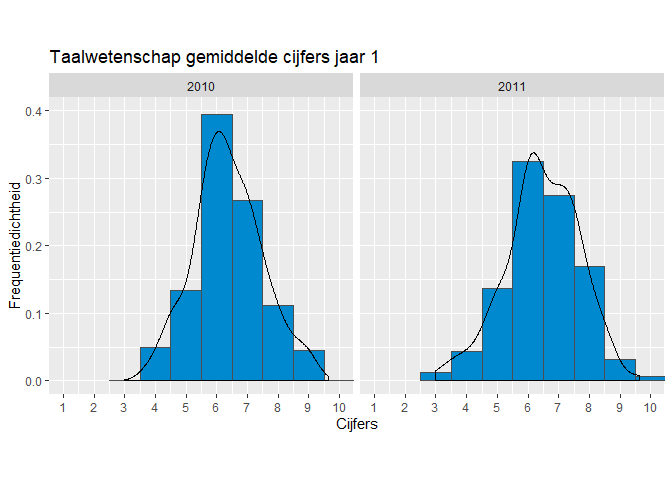
\includegraphics{01-One-sample-t-toets-R_files/figure-latex/histogram-1.pdf}

De histogram lijkt symmetrisch, heeft één top en geen outliers. De data
is dus bij benadering normaal verdeeld.

\hypertarget{q-q-plot}{%
\subsubsection{Q-Q plot}\label{q-q-plot}}

Gebruik \texttt{qqnorm()} en \texttt{qqline()} met \texttt{pch\ =\ 1}om
een Q-Q plot te maken, met als datapunten kleine cirkels.

Als over het algemeen de meeste datapunten op de lijn liggen, kan
aangenomen worden dat de data normaal verdeeld zijn.

\begin{Shaded}
\begin{Highlighting}[]
\CommentTok{## Q-Q plot}
\KeywordTok{qqnorm}\NormalTok{(Gemiddeld_cijfer_WNS, }
       \DataTypeTok{pch =} \DecValTok{1}\NormalTok{,}
       \DataTypeTok{main =} \StringTok{"Normaal Q-Q plot van gemiddelde cijfers WNS"}\NormalTok{,}
       \DataTypeTok{ylab =} \StringTok{"Kwantielen in data"}\NormalTok{,}
       \DataTypeTok{xlab =} \StringTok{"Theoretische kwantielen"}\NormalTok{)}
\KeywordTok{qqline}\NormalTok{(Gemiddeld_cijfer_WNS)}
\end{Highlighting}
\end{Shaded}

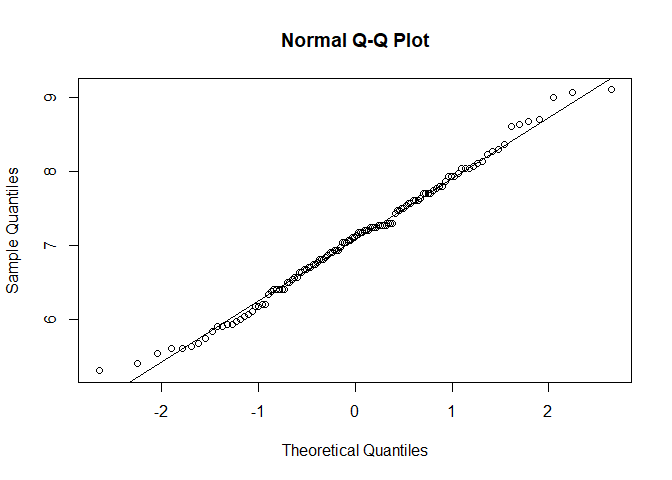
\includegraphics{01-One-sample-t-toets-R_files/figure-latex/qqplot-1.pdf}

In deze casus liggen de meeste punten op de lijn. Bij de uiteinden
liggen de punten dichtbij de lijn. Deze Q-Q plot duidt dus op een goede
benadering van de normaalverdeling.

\hypertarget{boxplot}{%
\subsubsection{Boxplot}\label{boxplot}}

De box geeft de middelste 50\% van de tentamencijfers weer. De zwarte
lijn binnen de box is de mediaan. In de staarten of snorreharen zitten
de eerste 25\% en de laatste 25\%.. Cirkels visualiseren mogelijke
uitbijters.\footnote{Outliers (13 augustus 2016).
  \href{https://wiki.uva.nl/methodologiewinkel/index.php/Outliers}{UvA
  Wiki Methodologiewinkel}.} Hoe meer de boxen overlappen, hoe
waarschijnlijker er geen significant verschil is tussen de groepen.

\begin{Shaded}
\begin{Highlighting}[]
\CommentTok{## Boxplot}
\KeywordTok{boxplot}\NormalTok{(Gemiddeld_cijfer_WNS, }\DataTypeTok{xlab =} \StringTok{"Werktuigbouwkunde"}\NormalTok{, }\DataTypeTok{ylab =} \StringTok{"Gemiddeld_cijfer_WNS"}\NormalTok{)}
\end{Highlighting}
\end{Shaded}

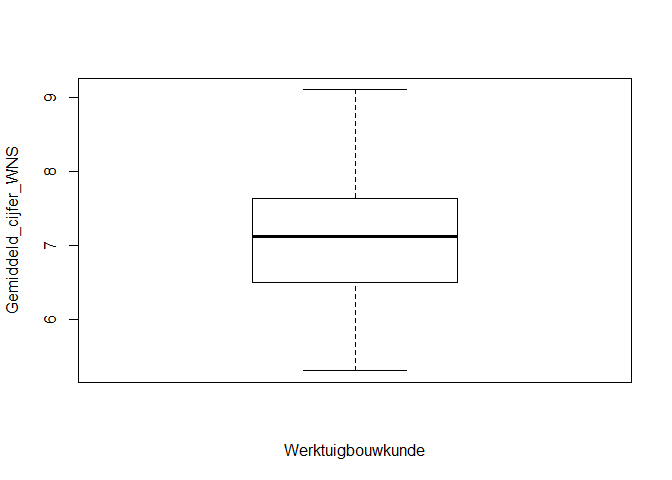
\includegraphics{01-One-sample-t-toets-R_files/figure-latex/boxplot-1.pdf}

De boxplot geeft de spreiding van het gemiddelde eindexamencijfer voor
de exacte vakken weer van de studenten Werktuigbouwkunde. De box en
staarten zien er symmetrisch uit, wat een indicatie is van een normale
verdeling.\footnote{Uitbijters kunnen bepalend zijn voor de uitkomst van
  toetsen. Bekijk of de uitbijters valide uitbijters zijn en niet een
  meetfout of op een andere manier incorrect verkregen data. Het
  weghalen van uitbijters kan de uitkomst ook vertekenen, daarom is het
  belangrijk om verwijderde uitbijters te melden in een rapport.}

\hypertarget{toetsen-van-normaliteit}{%
\subsection{Toetsen van normaliteit}\label{toetsen-van-normaliteit}}

Om te controleren of de data normaal verdeeld zijn, kan de normaliteit
getoetst worden. Twee veelgebruikte toetsen zijn: de
\emph{Kolmogorov-Smirnov test} en de \emph{Shapiro-Wilk test}.

\hypertarget{kolmogorov-smirnov}{%
\subsubsection{Kolmogorov-Smirnov}\label{kolmogorov-smirnov}}

De \emph{Kolmogorov-Smirnov test} toetst het verschil tussen twee
verdelingen. Standaard toetst deze test het verschil tussen een normale
verdeling en de verdeling van de steekproef.De Lilliefors correctie is
vereist als het gemiddelde en de standaardafwijking niet van tevoren
bekend of bepaald zijn, wat meestal het geval is bij een steekproef. Als
de p \textless{} 0,05 is, is de verdeling van de data statistisch
significant verschillend van de normale verdeling.

\begin{Shaded}
\begin{Highlighting}[]
\CommentTok{## Kolmogorov-Smirnov test}
\KeywordTok{library}\NormalTok{(nortest)}
\KeywordTok{lillie.test}\NormalTok{(Gemiddeld_cijfer_WNS)}
\end{Highlighting}
\end{Shaded}

\begin{verbatim}
## 
##  Lilliefors (Kolmogorov-Smirnov) normality test
## 
## data:  Gemiddeld_cijfer_WNS
## D = 0.041104, p-value = 0.8745
\end{verbatim}

De p-waarde is 0,87, dus er is geen statistisch significant verschil
gevonden tussen de verdeling van de steekproef en de normale verdeling.
De \emph{one sample-t-toets} kan uitgevoerd worden.

\hypertarget{shapiro-wilk-test}{%
\subsubsection{Shapiro-Wilk Test}\label{shapiro-wilk-test}}

De \emph{Shapiro-Wilk test} is een soortgelijke test als de
\emph{Kolmogorov-Smirnov test} en vooral geschikt bij kleine
steekproeven (n \textless{} 50). Als de p \textless{} 0,05 is, is de
verdeling van de data significant verschillend van de normale verdeling.
Er is een subset van \texttt{Gemiddeld\_cijfer\_WNS} ingeladen:
\texttt{Gemiddeld\_cijfer\_WNS\_n30}. De subset bevat 30 studenten. Voor
een relatief kleine steekproef als deze is de \emph{Shapiro-Wilk Test}
geschikt.

\begin{Shaded}
\begin{Highlighting}[]
\CommentTok{## Shapiro-Wilk test}
\KeywordTok{shapiro.test}\NormalTok{(Gemiddeld_cijfer_WNS_n30)}
\end{Highlighting}
\end{Shaded}

\begin{verbatim}
## 
##  Shapiro-Wilk normality test
## 
## data:  Gemiddeld_cijfer_WNS_n30
## W = 0.98159, p-value = 0.866
\end{verbatim}

De p-waarde is 0,87, dus er is geen statistisch significant verschil
gevonden tussen de verdeling van de steekproef en de normale verdeling.
De \emph{one sample-t-toets} kan uitgevoerd worden.

\hypertarget{one-sample-t-toets}{%
\subsection{One sample t-toets}\label{one-sample-t-toets}}

Gebruik \texttt{t.test()} om een t-toets uit te voeren. Gebruik het
argument \texttt{mu\ =\ 6.8} om het gemiddelde te specificeren waarmee
wordt vergeleken en specifieer welke alternatieve hypothese er getoetst
wordt. De verwachting is dat de studenten hoger scoren, maar omdat het
relevant is om te weten of de studenten ook lager scoren dan het
landelijk gemiddelde, is er voor gekozen om tweezijdig te toetsen.
Gebruik hiervoor \texttt{alternative\ =\ "two.sided"}. Gebruik de hele
dataset \texttt{Gemiddeld\_cijfer\_WNS} met \emph{n} = 124.

\begin{Shaded}
\begin{Highlighting}[]
\CommentTok{## T-test}
\KeywordTok{t.test}\NormalTok{(Gemiddeld_cijfer_WNS, }\DataTypeTok{mu =} \FloatTok{6.8}\NormalTok{, }\DataTypeTok{alternative =} \StringTok{"two.sided"}\NormalTok{)}
\end{Highlighting}
\end{Shaded}

\begin{verbatim}
## 
##  One Sample t-test
## 
## data:  Gemiddeld_cijfer_WNS
## t = 4.6634, df = 123, p-value = 7.97e-06
## alternative hypothesis: true mean is not equal to 6.8
## 95 percent confidence interval:
##  6.989216 7.268311
## sample estimates:
## mean of x 
##  7.128763
\end{verbatim}

\begin{itemize}
\tightlist
\item
  Vrijheidsgraden, \emph{df} = \emph{n} -1 = 124-1 = 123\\
\item
  \emph{t} \textsubscript{123} = 4,66, \emph{p} \textless{} 0,0001
\item
  p-waarde \textless{} 0,05, dus de H\textsubscript{0} wordt verworpen
  \footnote{In dit voorbeeld wordt uitgegaan van een waarschijnlijkheid
    van 95\% c.q. een p-waardegrens van 0,05. De grens is naar eigen
    inzicht aan te passen; houd hierbij rekening met type I en type II
    fouten.}
\item
  95\%-betrouwbaarheidsinterval: bij het herhalen van het experiment met
  verschillende steekproeven van de populatie zal 95\% van de
  betrouwbaarheidsintervallen de daadwerkelijke parameter bevatten, het
  gemiddeld eindexamencijfer exacte vakken. In deze casus is het
  interval tussen 6,99 en 7,27. Aangezien 6.8 niet in dit interval zit,
  verschilt het gemiddelde significant van 6.8.
\item
  Het gemiddelde van de steekproef is 7,13 
\end{itemize}

\hypertarget{rapportage}{%
\section{Rapportage}\label{rapportage}}

De \emph{one sample t-toets} is uitgevoerd om te toetsen of het
gemiddelde eindexamencijfer voor de exacte vakken van vwo studenten die
Werktuigbouwkunde zijn gaan studeren anders is dan het landelijk
gemiddelde. Het gemiddelde van de steekproef (\emph{M} = 7,13, \emph{SD}
= 0,79) is significant verschillend van het landelijk gemiddelde van
6,8, \emph{t} \textsubscript{123} = 4,66, \emph{p} \textless{} 0,0001.
De resultaten ondersteunen de conclusie dat het gemiddelde
eindexamencijfer voor de exacte vakken van studenten Werktuigbouwkunde
met een vwo vooropleiding hoger ligt dan het landelijk gemiddelde.

\leavevmode\hypertarget{footer}{}%
Deze pagina maakt onderdeel uit van het Statistisch Handboek Studiedata,
ontwikkeld binnen de zone Veilig en betrouwbaar benutten van studiedata
van het Versnellingsplan. R code is uitgevoerd met R versie 3.6.3;
Python code is uitgevoerd in Python 3.7. © 2020 Versnellingsplan -
Statistisch Handboek Studiedata - Licentie Laatst gewijzigd
op:25-05-2020

\end{document}
